\documentclass[]{report}
\usepackage{pdfpages}
%\usepackage{amsmath}


\usepackage{listings}
\usepackage{xcolor}

\colorlet{punct}{red!60!black}
\definecolor{background}{HTML}{EEEEEE}
\definecolor{delim}{RGB}{20,105,176}
\colorlet{numb}{magenta!60!black}

\lstdefinelanguage{json}{
    basicstyle=\normalfont\ttfamily,
    numbers=left,
    numberstyle=\scriptsize,
    stepnumber=1,
    numbersep=8pt,
    showstringspaces=false,
    breaklines=true,
    frame=lines,
    backgroundcolor=\color{background},
    literate=
     *{0}{{{\color{numb}0}}}{1}
      {1}{{{\color{numb}1}}}{1}
      {2}{{{\color{numb}2}}}{1}
      {3}{{{\color{numb}3}}}{1}
      {4}{{{\color{numb}4}}}{1}
      {5}{{{\color{numb}5}}}{1}
      {6}{{{\color{numb}6}}}{1}
      {7}{{{\color{numb}7}}}{1}
      {8}{{{\color{numb}8}}}{1}
      {9}{{{\color{numb}9}}}{1}
      {:}{{{\color{punct}{:}}}}{1}
      {,}{{{\color{punct}{,}}}}{1}
      {\{}{{{\color{delim}{\{}}}}{1}
      {\}}{{{\color{delim}{\}}}}}{1}
      {[}{{{\color{delim}{[}}}}{1}
      {]}{{{\color{delim}{]}}}}{1},
}


\begin{document}
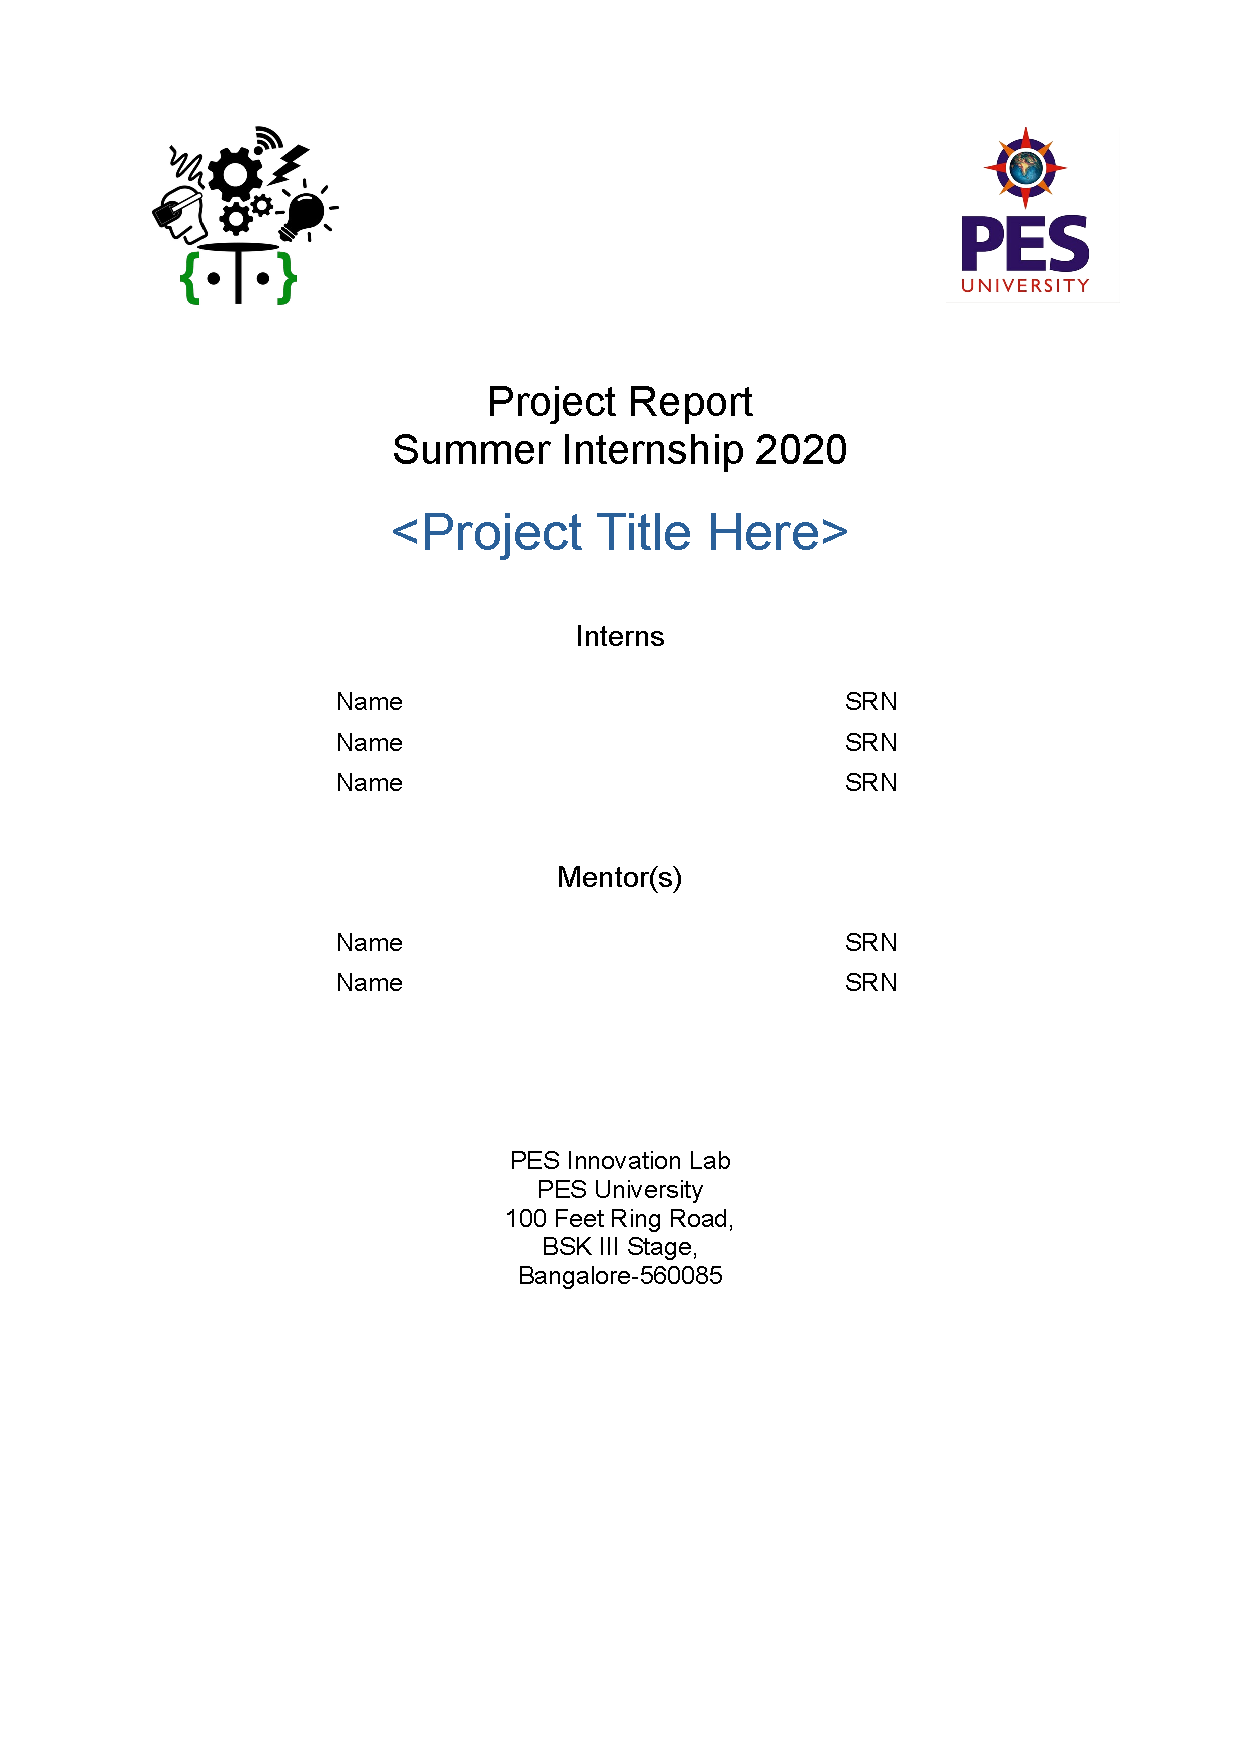
\includepdf[pages={1}]{coverpage.pdf} 

\begin{abstract}
 In recent years, the significant increase in air pollution is a major topic of discussion among the public, government, academia and air pollution experts. There is no doubt that keeping the air clean and protecting it from various sources of emissions is essential to the survival oh life on Earth and is a major global issues and concern for any government. The quality of urban environment directly affects people's health, and it is important to understand the real-time status of urban air quality. AQVis aims to successfully aggregate the Air Quality Data generated by the sensors on the cloud and obtaining meaningful visualizations and insights. This report on AQVis aims to design and implement a cloud based management system to store and visualize the data brought in from the sensors.
\end{abstract}

\tableofcontents
\listoffigures
\listoftables



\chapter{Introduction}

\section{Background}
Students and Faculty from PES University are currently working on developing Air Quality sensors that can be used to detect the particulate matter concentration of pollutants around where they are placed. These devices consist of three individual sensors, each of which is detecting the count of particulate matter that are 2.5, 7.5 and 10 micrometers or less in diameter. These devices will send the data obtained by the sensors to a cloud based system that stores and analyzes the data along with other information such as the battery level, location and timestamp.

\section{Problem Statement}
This project (AQVis) aims to be the Cloud based counterpart to the Air Quality sensors. The data that is obtained from the sensors is passed onto the Cloud based servers that are capable of ingesting the data sent by the devices and store it in a secure and accessible manner. A dashboard created must house relevant visualizations and maps to generate useful insights from the data.

\section{Application}
The cloud based system and dashboard will be used to convey information about air quality to users. Currently, there very number of limited air quality sensors in India. This project aims to make sensors more widespread to enable the accurate tracking of air pollution parameters. Using this data, insights can be gained on the spread of pollution and trends in particulate matter concentration.

 

\chapter{Literature Survey/Related Work} 

\section{Existing Solutions}
There are multiple online air quality monitoring websites that have been referred to throughout the course of this project.

\subsection{PurpleAir}
PurpleAir\cite{purpleair} is a brand of air quality sensors that can be purchased and installed at any location. They connect to the server via wifi and monitor multiple different sizes of particulate matter. The online dashboard of PurpleAir shows a map with a point at the location of each sensor. The point displays a color according to the health safety and a number corresponding to an average sensor measurement. The map can be interacted with to locate different sensors. Upon clicking on a sensor, a graph displaying data from that sensor is displayed. We found this user interface very easy to use and have used it as a reference in our final design.

\subsection{Aqandu}
Aquandu\cite{aqandu} is an air quality monitoring dashboard that procures data from already placed sensors. It has been created by researchers at the University of Utah and centres the data around Salt Lake City. The data on Aquandu is sourced from four different types of sensors. The map is in black and white and a fixed graph with the data from the selected sensor is displayed at the bottom. The University of Utah has also used the data accumulated to model and forecast pollution data.\cite{aqandu:mlvideo} Attempting something similar to this is part of the future scope for this project.

\section{Novelty of Work}
The solution proposed in this project is similar to the above mentioned examples in the basic approach. A map along with graphs for the selected sensors will be prominently displayed on the application. A unique feature that will stands out and that set this solution apart is the presence of moving sensors. Having sensors that constantly change their location results in a larger number of variables and unique computations to visualize information. This feature has not been implemented in the above mentioned solutions. Having a custom built server and dashboard will allow greater autonomy over the processing and storage of data along with better control over data analysis. Parameters and functions can be instantly tweaked according to the sensor's evolving capabilities which is difficult to accomplish with an existing solution.



\chapter{Approach}
After thorough research and trials, the approach decided on was to develop an API server using Flask to handle the incoming requests from the sensor devices. The Elastic stack formerly known as ELK stack comprising of Elasticsearch, Logstash and Kibana is used to handle and visualize the data. Elasticsearch is used as the database and Kibana is used to visualize the data. The front-end comprises of OpenLayers used to generate maps. A custom dashboard is built consisting of the graphs from Kibana and OpenLayers maps that will face the user. Using Kibana for the graphs allows them to be dynamic and easily modifiable which results in users being able to tweak the views to their specifications. The flow of data from sensors to the users is depicted in Figure \ref{dataflow}. Message Queues are a feature we expect to add in the future to reduce the load on our server and streamline data ingestion. All the software used in this project was hosted on virtual machines using Google Cloud Platform. The flow of users in the applications is depicted in \ref{userflow}.

\begin{figure}[ht]
  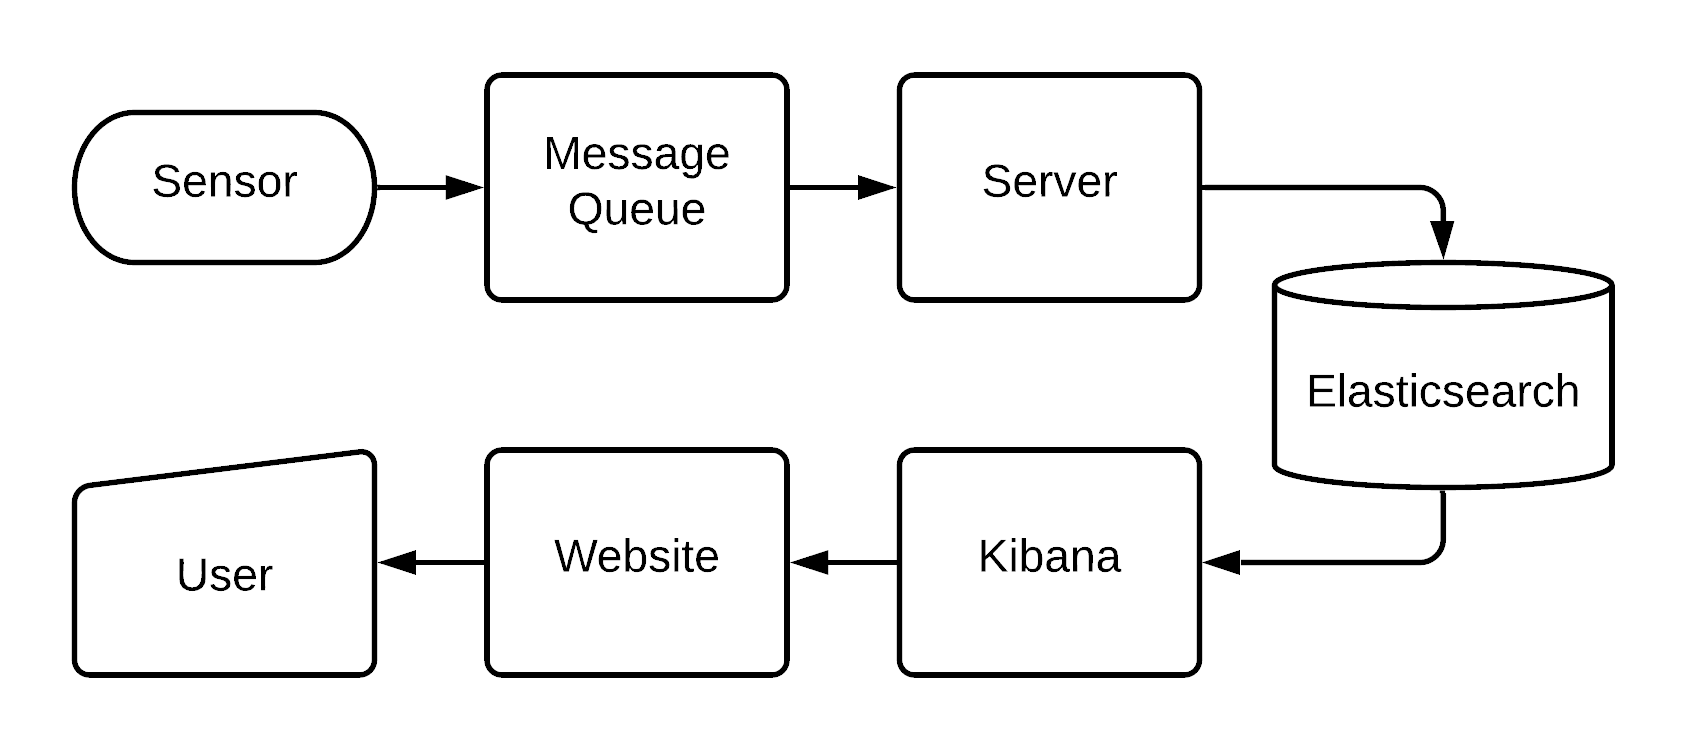
\includegraphics[width =\columnwidth]{dataflow.png}
  \caption{Data Flow Chart}
  \label{dataflow}
\end{figure}

\begin{figure}[ht]
  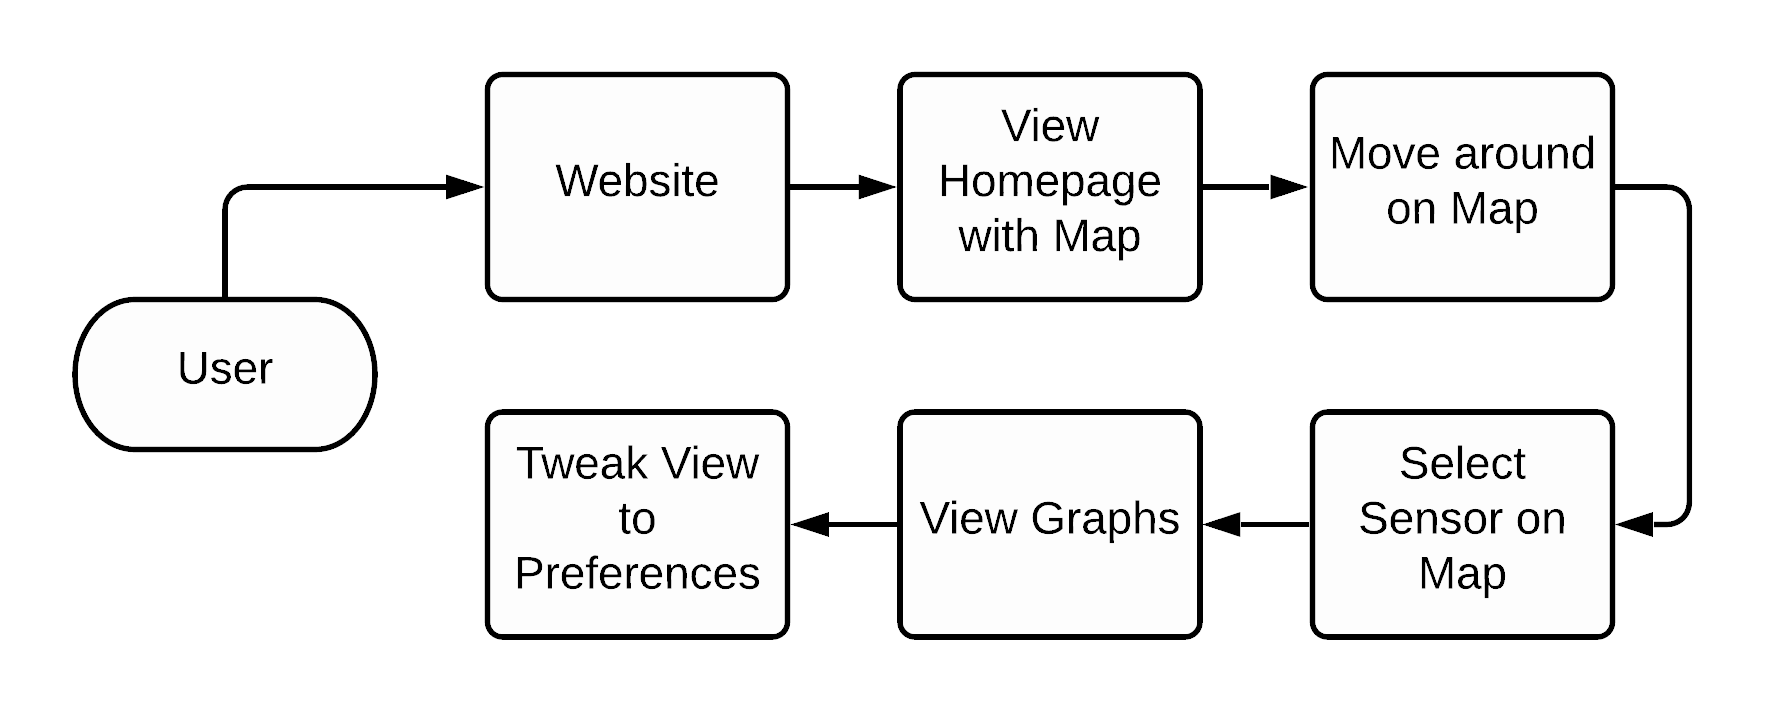
\includegraphics[width =\columnwidth]{userflow.png}
  \caption{User Flow Chart}
  \label{userflow}
\end{figure}

\section{Database}
One of the most pivotal parts to this project was the logging of data that is received from the sensors. This calls for a database management system that will suit this need accordingly. There are two major classifications when it comes to database selection .viz SQL based and NoSQL based.

\subsection{SQL Based}
Relational databases store data sets as “relations”: tables with rows and columns where all information is stored as a value of a specific cell. Data in an RDBMS is managed using SQL. Though there are different implementations, SQL is standardized and provides a level of predictability and utility.
Relational databases excel at handling highly structured data and provide support for ACID (Atomicity, Consistency, Isolation, and Durability) transactions. Data is easily stored and retrieved using SQL queries
The biggest weakness of relational databases is the mirror of their biggest strength. As good as they are at handling structured data, they have a hard time with unstructured data.

\subsection{NoSQL based}
Even though many applications use an SQL database for logging, it is not highly efficient to store data from a logging workload. Logs don’t require UPDATE/DELETE or rollback and can be considered as an append-only workload. Using a database engine that is designed to support OLTP workload is a missed opportunity to use a more specialized storage solution. Taking all the above into account, the Elastic Stack seemed to be the best fit for this project's needs.


\section{Front-end}
Front-end development is a practice that enables creation of an intuitive and concentric user experiences for web applications or website. It is important that the front-end is highly user friendly and dynamic. The front-end consists of a website built primarily in HTML, CSS and JavaScript. The application uses the Openlayers API to render map vector tiles on the website. Additional maps are included using API keys from other sources like BING maps, etc. Graphs and related visualizations are obtained and embedded from Kibana.


\chapter{Implementation}

\section{Infrastructure Requirements}

\begin{table}[ht]
\label{hardware}
\begin{center}
\begin{tabular} {l|l|l} %left aligned
\hline
\hline
\textbf{Virtual Machine Instance} & \textbf{Operating System} & \textbf{Specifics}  \\
\hline
Data Ingestion Server & Debian 10 & 1 vCPU, 3.75 GB \\
ELK Server & Debian 10 & 1 vCPU, 3.75 GB \\
Frontend Server & Debian 10 & 1 vCPU, 3.75 GB \\
\hline 
\hline
\end{tabular}
\end{center}
\caption{Virtual Machine Details}
\end{table}


\section{Software Requirements}

\begin{table}[ht]
\label{software}
\begin{center}
\begin{tabular} {l|l} %left aligned
\hline
\hline
\textbf{Software Name} & \textbf{Version Number} \\
\hline
Python & 3.7.6 \\
Gunicorn & 19.9.0 \\
Flask & 1.1.2 \\
Elastic Stack & 7.7 \\
ol (OpenLayers) & 6.3.1 \\
ol-parcel & 1.0.0\\
dist & 0.1.2 \\
ol-ext & 3.1.12 \\
ol-geocoder & 4.0.0 \\
parcel-bundler & 1.9.4\\
\hline 
\hline
\end{tabular}
\end{center}
\caption{Software Details}
\end{table}


\section{Software}
\subsection{Elastic Stack}
Elastic Stack\cite{"elastic"} , formerly known as ELK stack is a group of open source products that help help users take data from any type of source and in any format and search, analyze, and visualize that data in real time. This can be deployed on the fully hosted and supported service by Elastic.org on their cloud service, ELK Cloud or as a standalone version on a local machine or a cloud service like this project does. 
\newline
\newline
\begin{figure}[ht]
    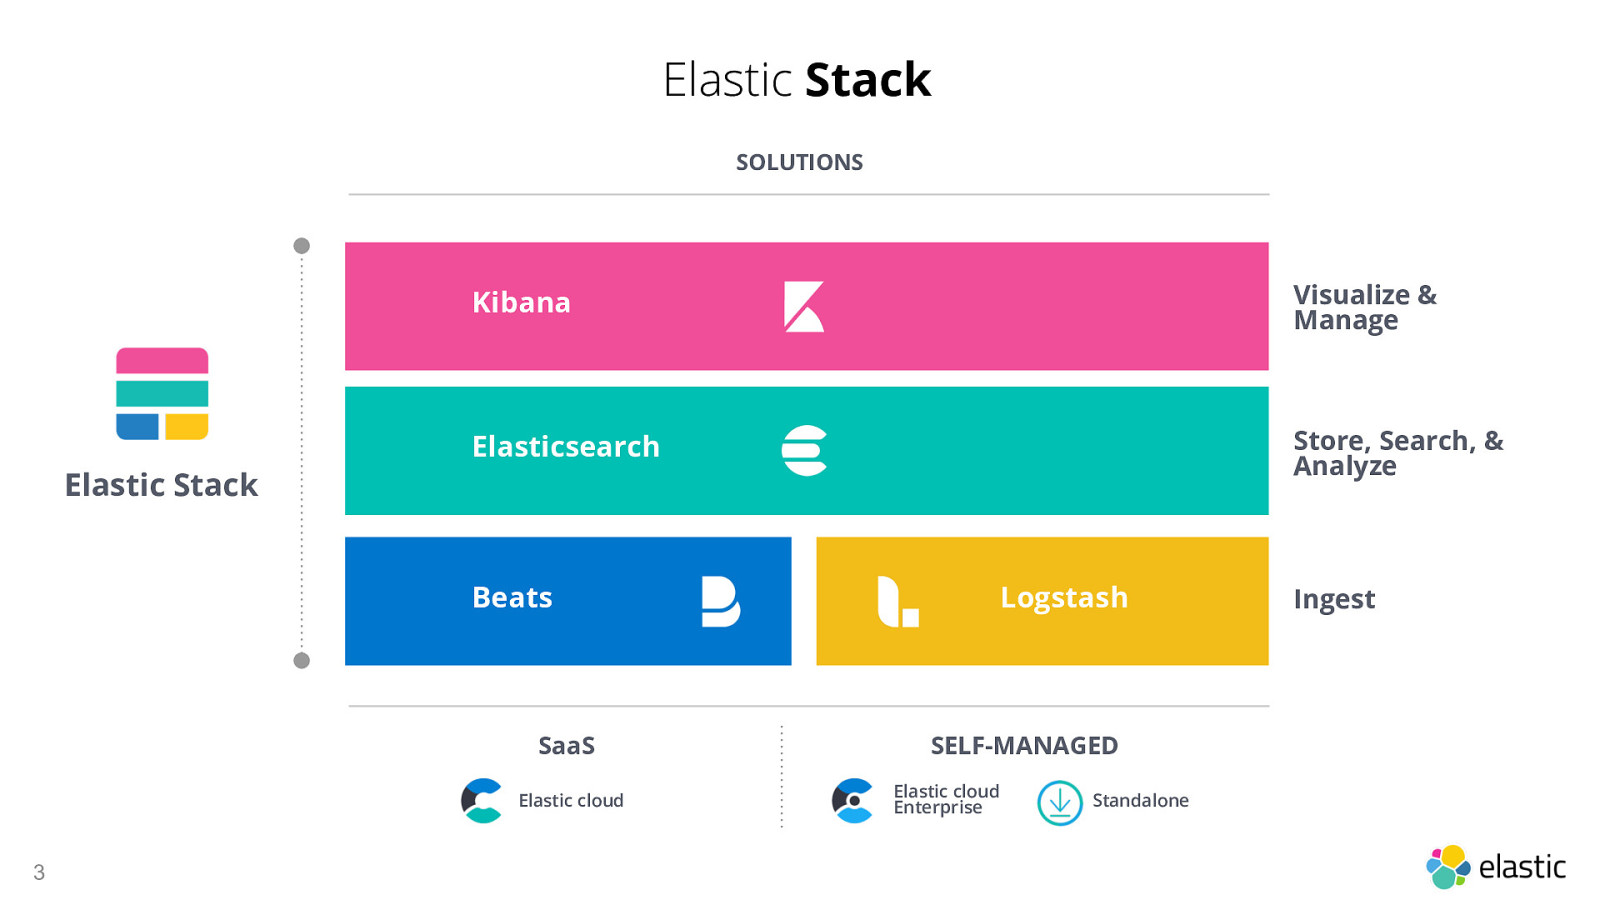
\includegraphics[width =\columnwidth]{elastic_framework.jpg}
    \caption{Elastic stack framework}
    \label{fig:elastic_framework}
\end{figure}
Elastic Stack components:
\begin{enumerate}
    \item 
    Elasticsearch is a RESTful distributed search engine built on top of Apache Lucene and released under an Apache license. It is Java-based and can search and index document files in diverse formats.
    \item
    Logstash is a data collection engine that unifies data from disparate sources, normalizes it and distributes it. The product was originally optimized for log data but has expanded the scope to take data from all sources
    \item
    Beats are “data shippers” that are installed on servers as agents used to send different types of operational data to Elasticsearch either directly or through Logstash, where the data might be enhanced or archived.
    \item
    Kibana is an open source data visualization and exploration tool from that is specialized for large volumes of streaming and real-time data. The software makes huge and complex data streams more easily and quickly understandable through graphic representation
\end{enumerate}
\begin{figure}[h]
    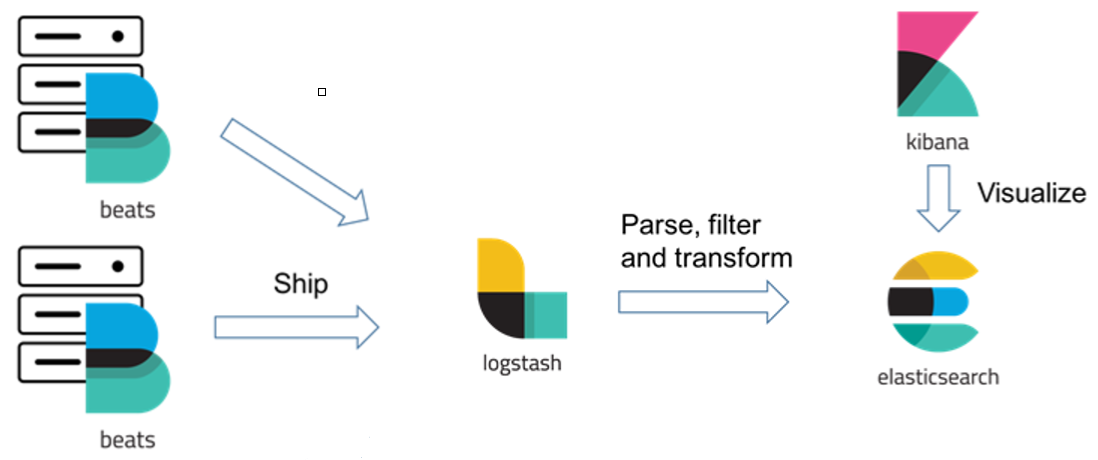
\includegraphics[width =\columnwidth]{elasticflow.png}
    \caption{Flow of data in elastic stack}
    \label{fig:elasticflow}
\end{figure}


\subsection{Openlayers}
OpenLayers\cite{"Openlayers"} is a bundled API that makes it easy to put a dynamic map in any web page. It can display map tiles, vector data and markers loaded from any source. OpenLayers has been developed to further the use of geographic information of all kinds.With the help of parcel bundler it Bundles all the webpages present into a production ready static files.

\subsection{Parcel}
Parcel is a web application bundler, differentiated by its developer experience.It can take any type of file as an entry point, but an HTML or JavaScript file is a good place to start. If you link your main JavaScript file in the HTML using a relative path, Parcel will also process it for you, and replace the reference with a URL to the output file.


\subsection{Flask}
The server handling the ingestion of data from the sensor devices was written in Python using the Flask framework. Two API routes were created, one for adding a new device and one for adding data from a device. The Flask server was used while testing.

\subsection{Gunicorn}
Due to the Flask server being solely for development purposes, Gunicorn was used as the production server.

\section{Data Format}
The format of data sent from the sensors was finalized after collaborating with the sensor development team. The data will be sent in the POST requests sent through Hyper Text Transfer Protocol (HTTP). The format used to send the data is JSON. The format and datatypes of the individual values are listed below. The timestamp sent by the device is of the form hh:mm:ss.

\begin{lstlisting}[language=json,firstnumber=1]
{
    "device_id": string,
    "timestamp": string,
    "altitude": float,
    "latitude": float,
    "longitude": float,
    "battery_level": float,
    "aq1": {
        "pm10": float,
        "pm75": float,
        "pm25": float
    },
    "aq2": {
        "pm10": float,
        "pm75": float,
        "pm25": float
    },
    "aq3": {
        "pm10": float,
        "pm75": float,
        "pm25": float
    }
}
\end{lstlisting}

The same data received by the flask server from the senors is parsed, verified and sent to the Elasticsearch database. Minor additions to the data include the date, which is not sent by the sensor device. The latitude and longitude are included in a single object named location in order to allow Elasticsearch to index it as a geo-spatial value. When a new device creation request is sent, flask needs to create a new index in Elasticsearch and specify the timestamp format. This allows Elasticsearch to index the timestamp field correctly.

\chapter{Results and Discussion}
\section{Webpage}
Using Openlayers\cite{"Openlayers"} to display the map and Kibana\cite{"elastic"} for the visualisation along with other APIs , a basic front end user interface is obtained as shown in figure \ref{fig:Basic Frontend}

\begin{figure}[ht]
    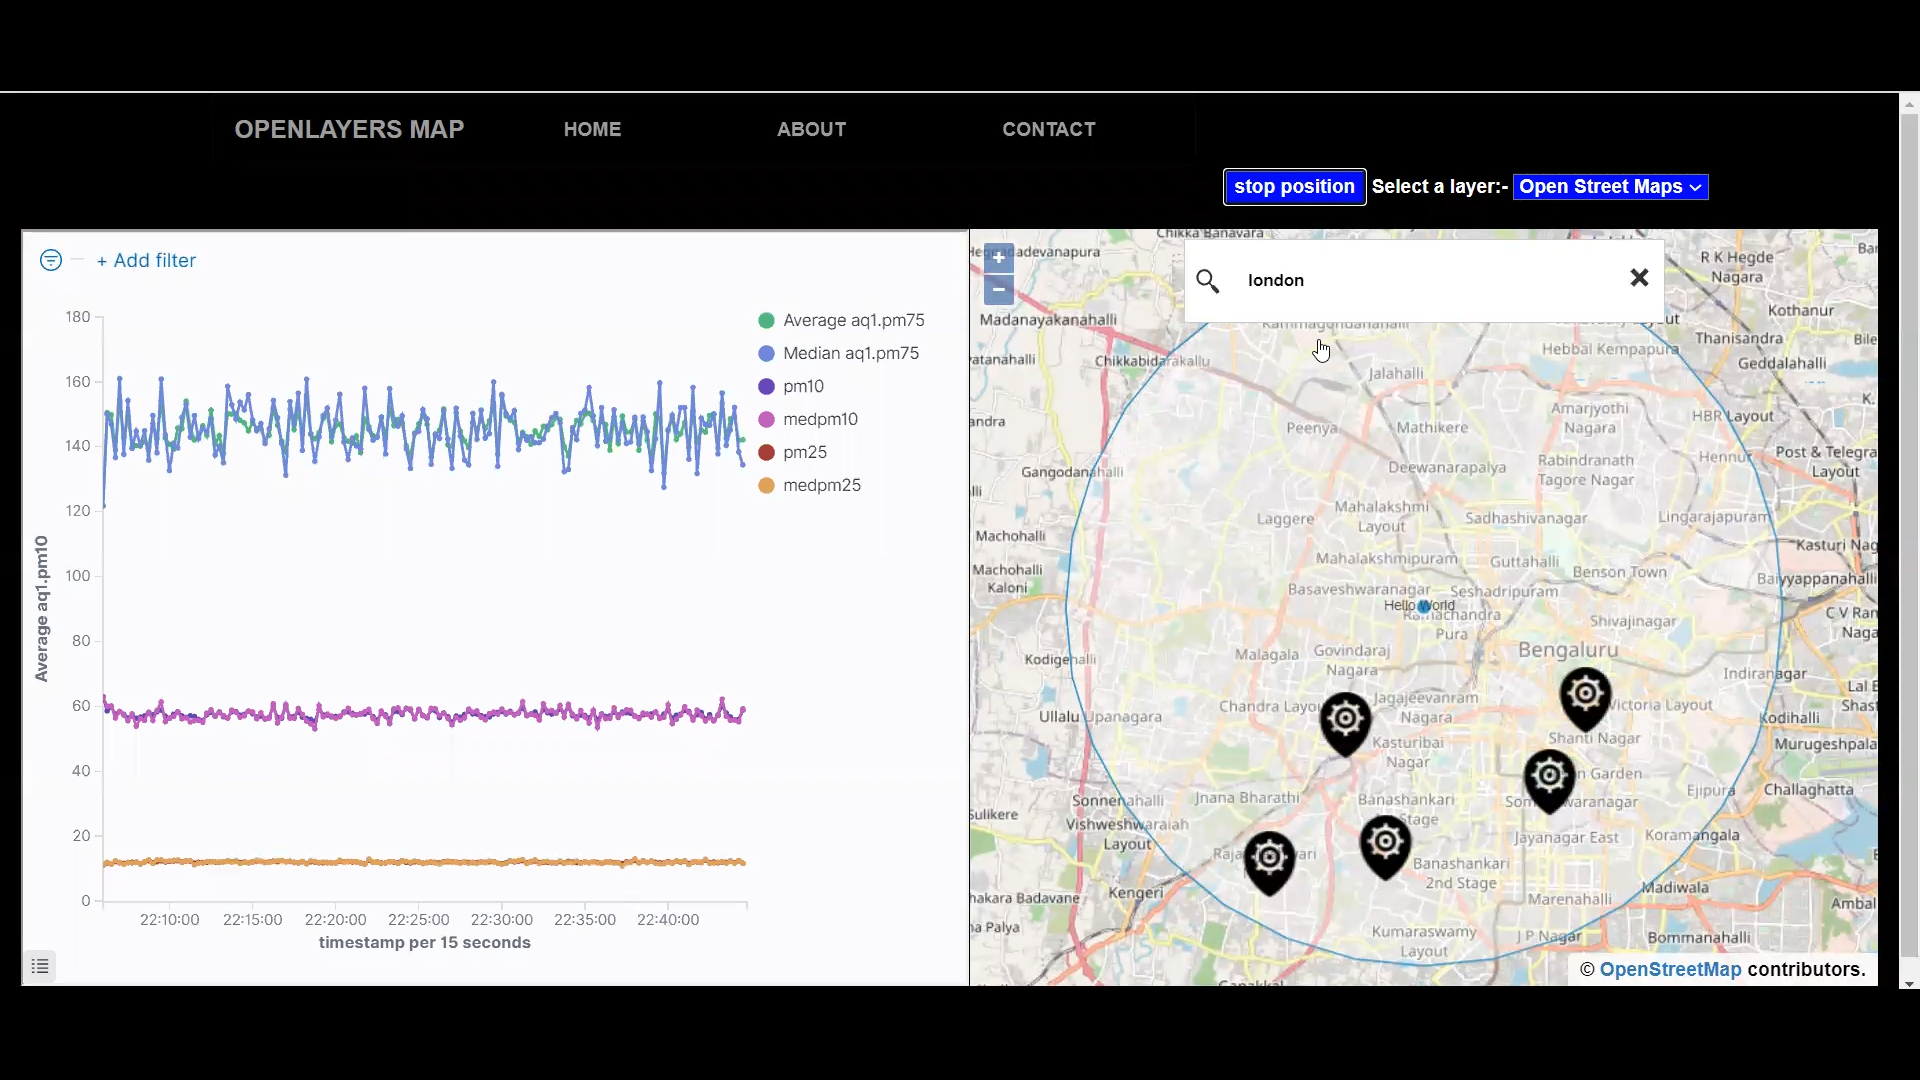
\includegraphics[width =\columnwidth]{frontend.png}
    \caption{Basic Frontend}
    \label{fig:Basic Frontend}
\end{figure}
\newpage
\subsection{Using the webpage}
When the page loads onto the browser window, the user needs to click on any of the markers present on the map and the graph pops up displaying the analysed data in a easy to comprehend manner for the user.



%Include tables (see Table \ref{XYComparison} for a template), figures and plots to represent your results if possible. What were the key outcomes? Do they match with expected results? Why/why not? Discuss and explain results where possible. Talk about challenges faced and the limitations of the present implementation if any. 


\chapter{Conclusions and Future Work}
\section{Conclusion}
Air quality and the state of the environment was and will continue to be an ever growing concern for mankind. This project will do it's part to help in the visualisation and analysis of air quality so that appropriate actions can be taken.
\section{Future Scope}
The possibilities of collaborations, future developments and improvements on this project are endless. Some of the future scopes for this include but are not limited to the following:
\newline
\begin{itemize}
    \item A customize-able visualisation dashboard for the user to use
    \item Air quality prediction models that make smart predictions. 
    \item Mobile sensor technology mounted on vehicles 
    \item Route recommendation based on lesser pollution 
    \item Heat map based display for pollution comparison 

\end{itemize}



\bibliographystyle{ieeetr} 
\bibliography{bibmil.bib}
\appendix 
\chapter{Kibana visualisations}
\section{Kibana dashboard examples}
\begin{figure}[ht]
    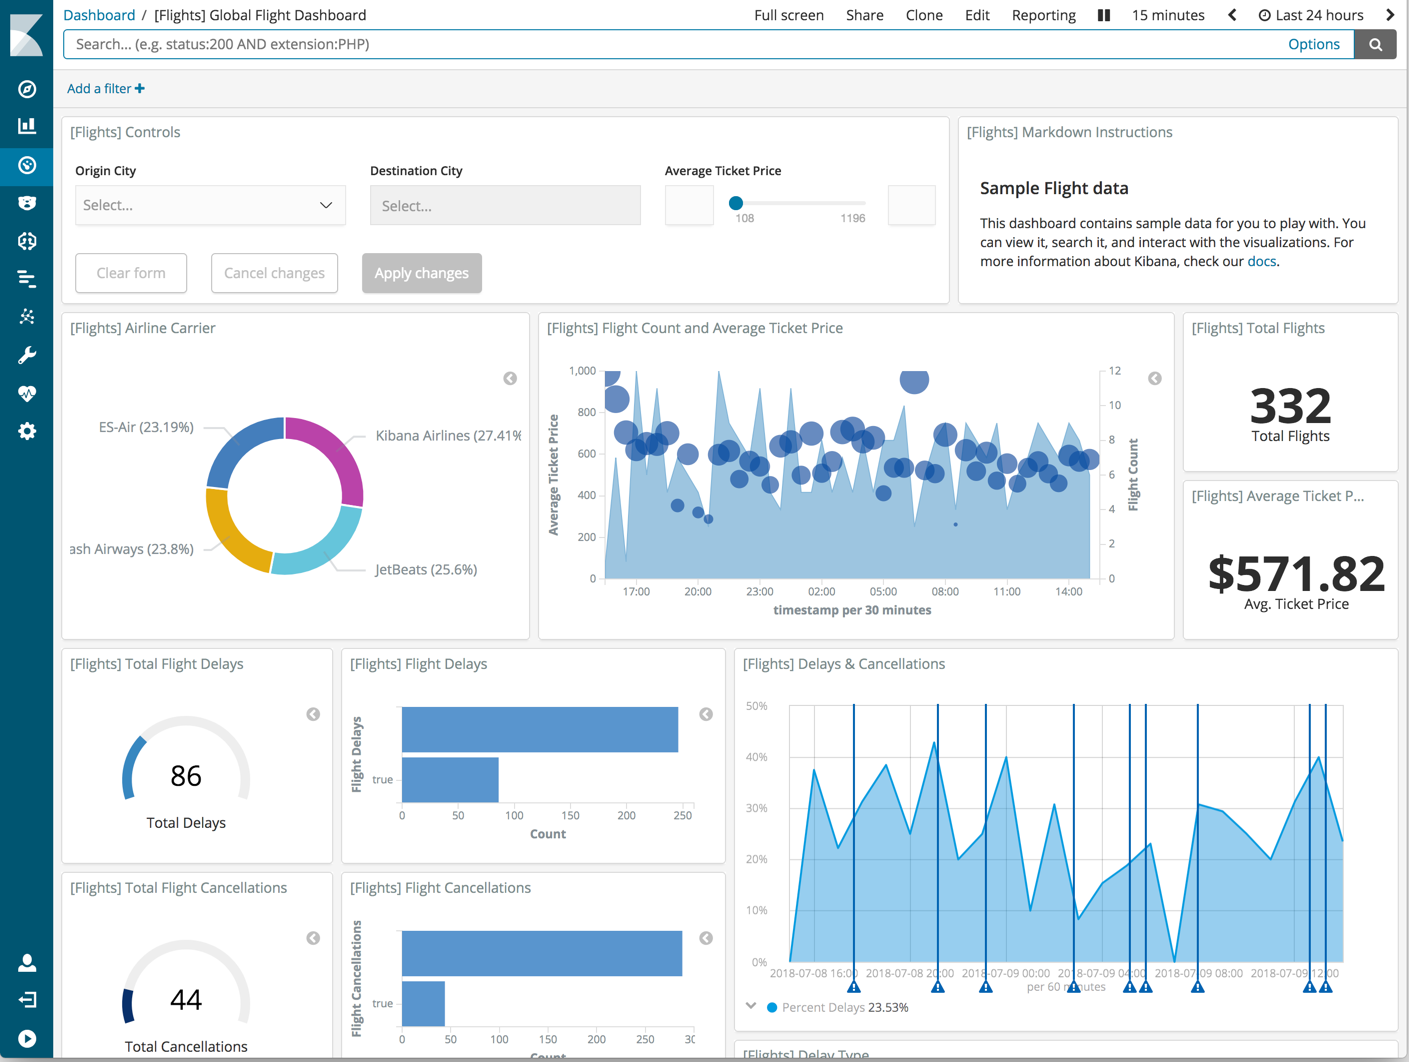
\includegraphics[width =\columnwidth]{dashboard_example1.png}
    \caption{Example 1}
    \label{fig:EX1}
\end{figure}
\begin{figure}[ht]
    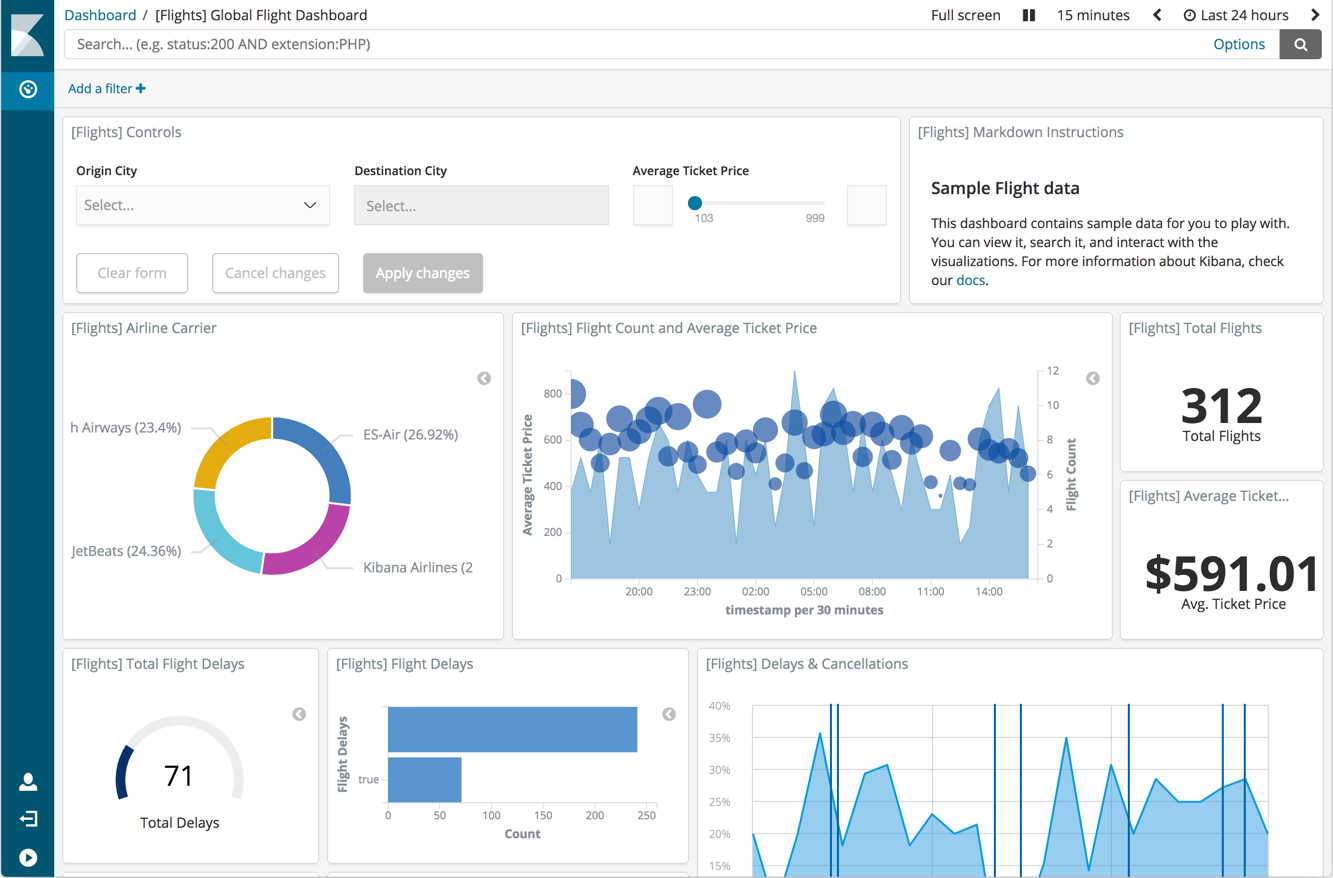
\includegraphics[width =\columnwidth]{dashboard_example2.png}
    \caption{Example 2}
    \label{fig:EX2}
\end{figure}
\begin{figure}[ht]
    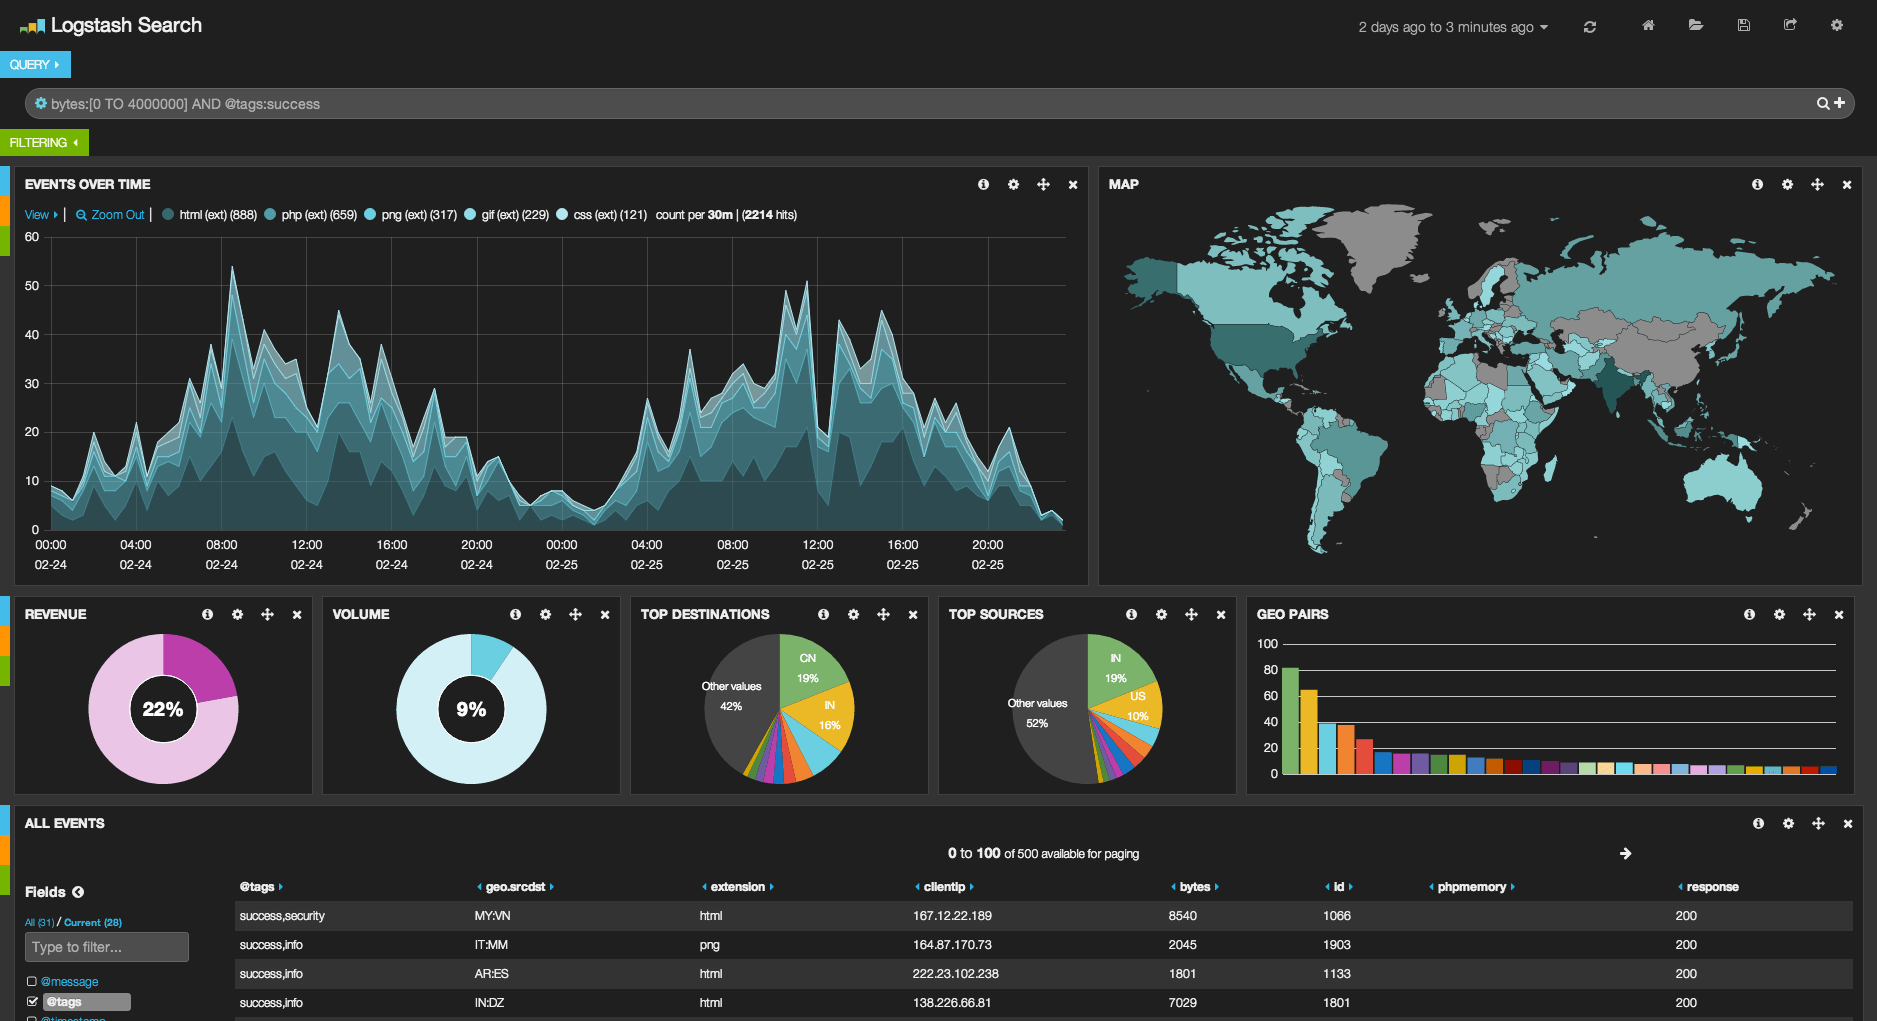
\includegraphics[width =\columnwidth]{dashboard_example3.png}
    \caption{Example 3}
    \label{fig:EX3}
\end{figure}
\begin{figure}[ht]
    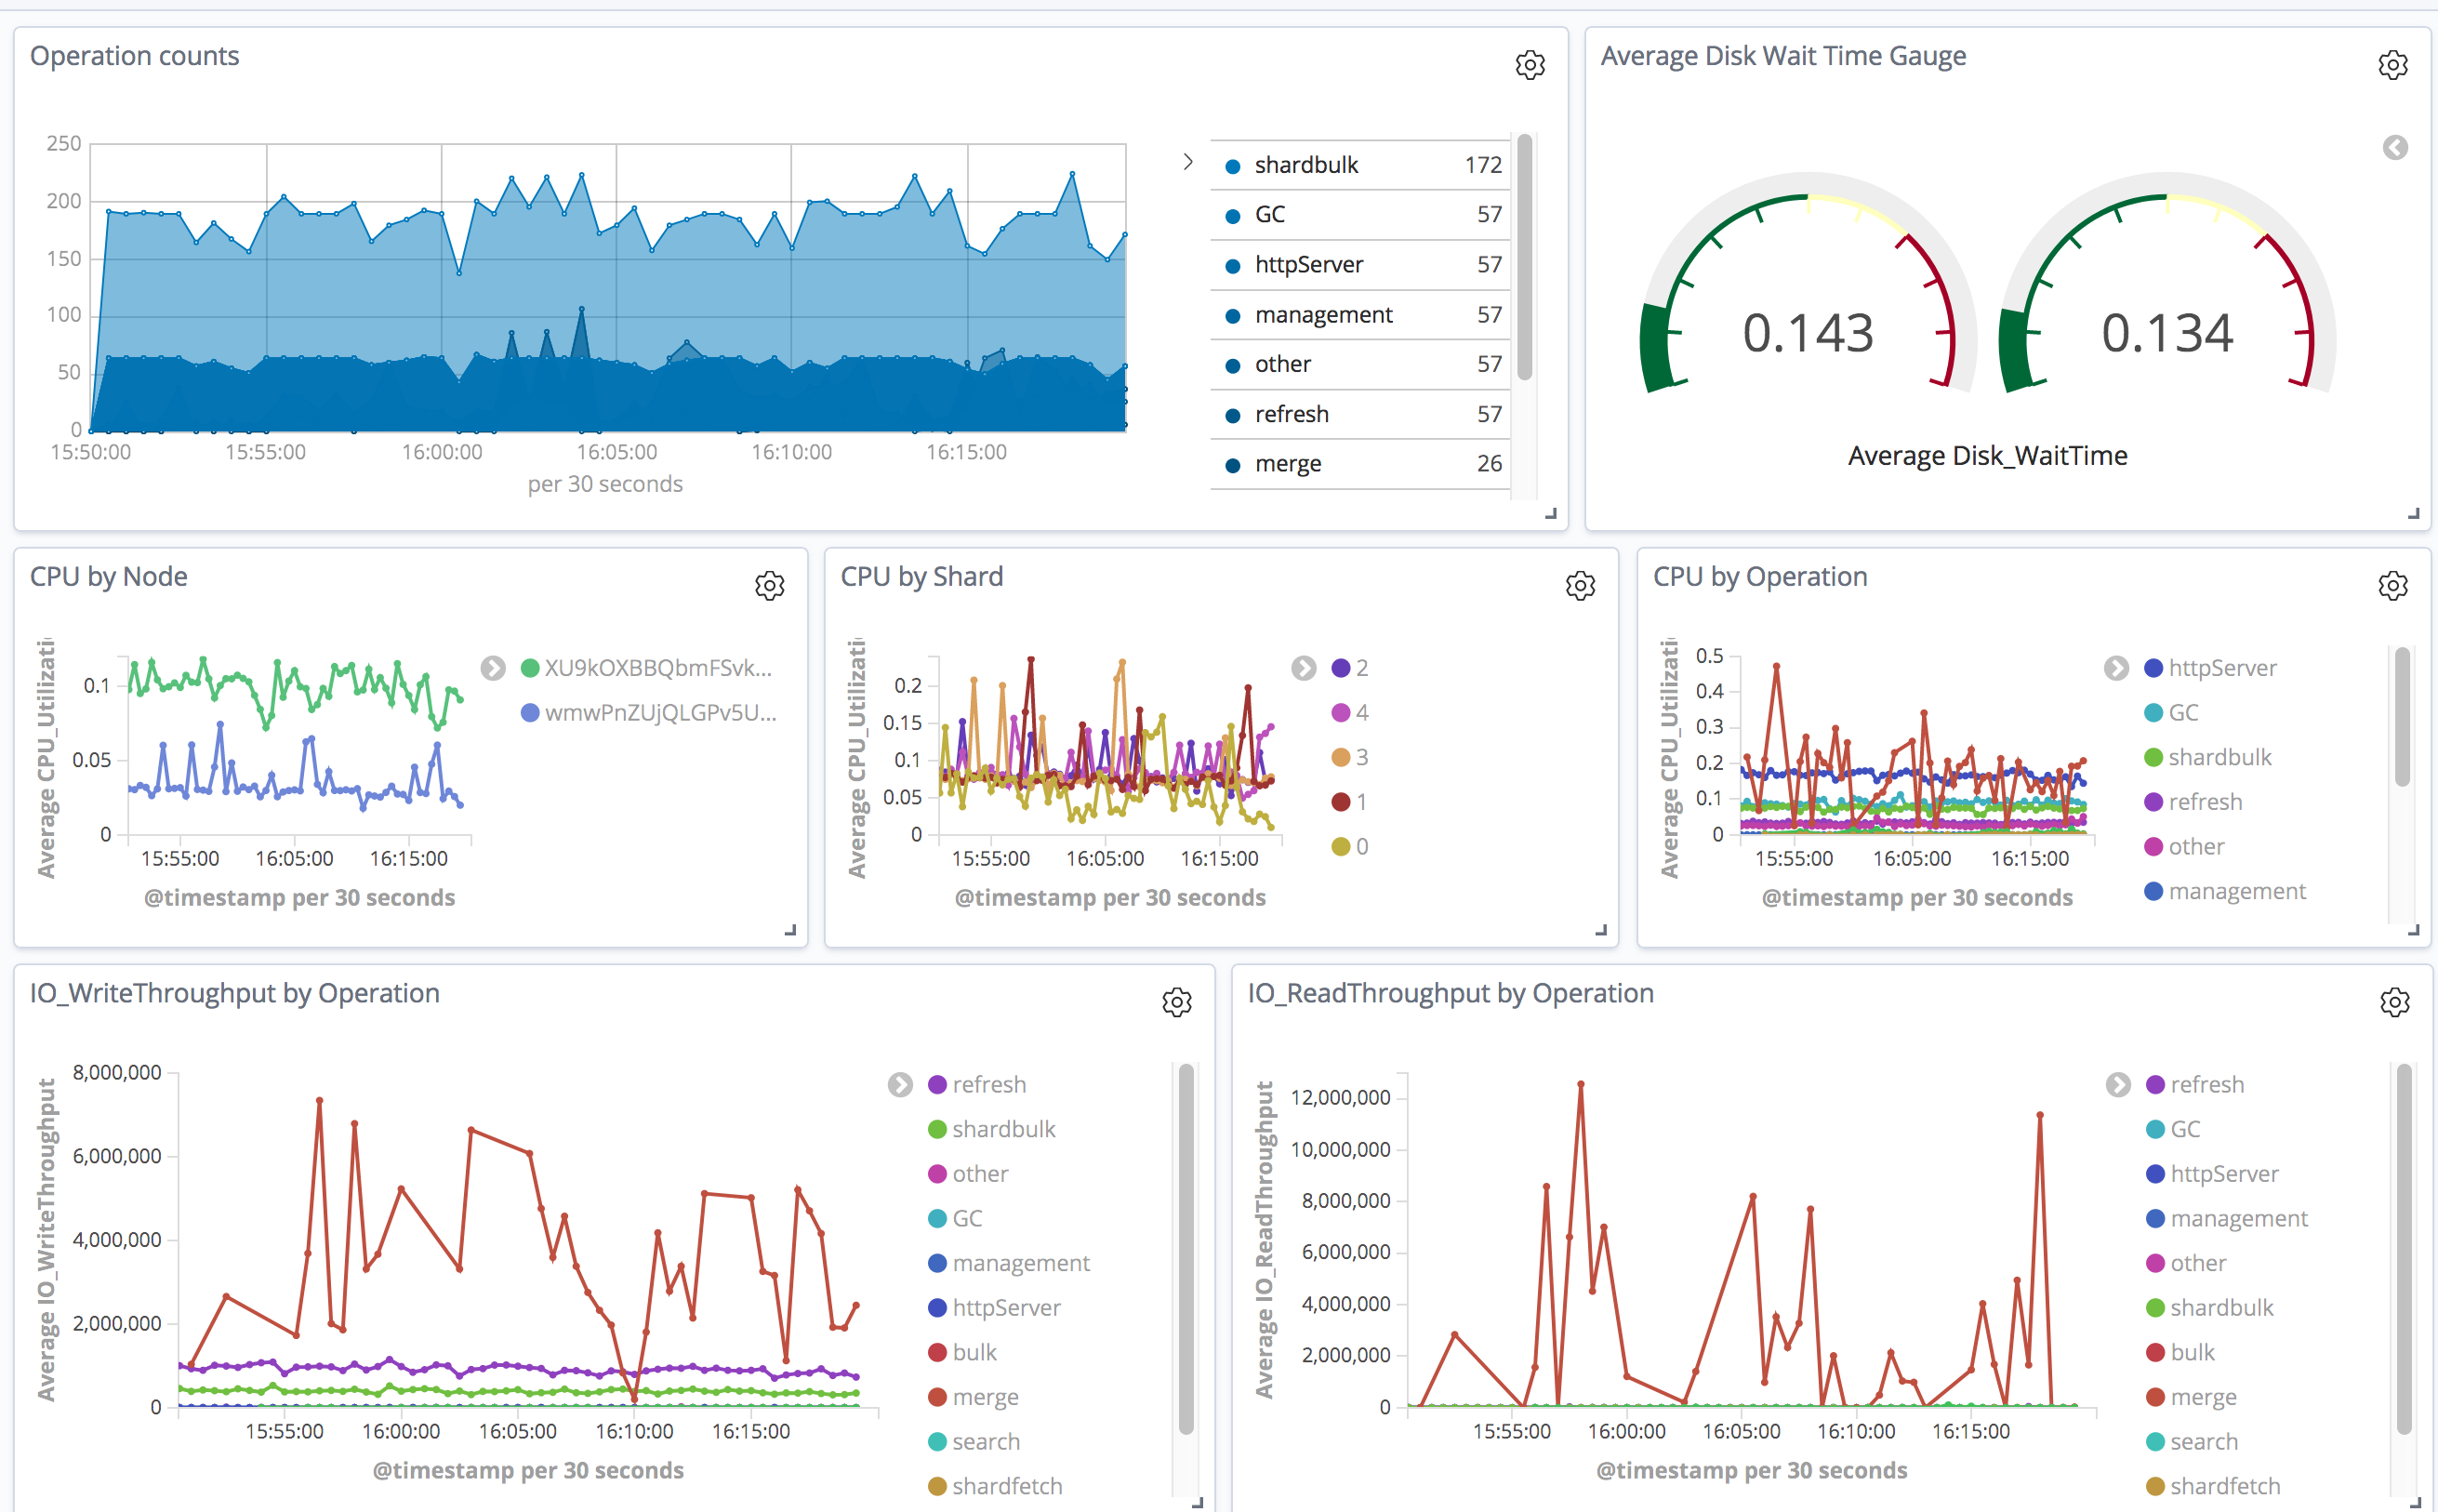
\includegraphics[width =\columnwidth]{dashboard_example4.png}
    \caption{Example 4}
    \label{fig:EX4}
\end{figure}
\begin{figure}[ht]
    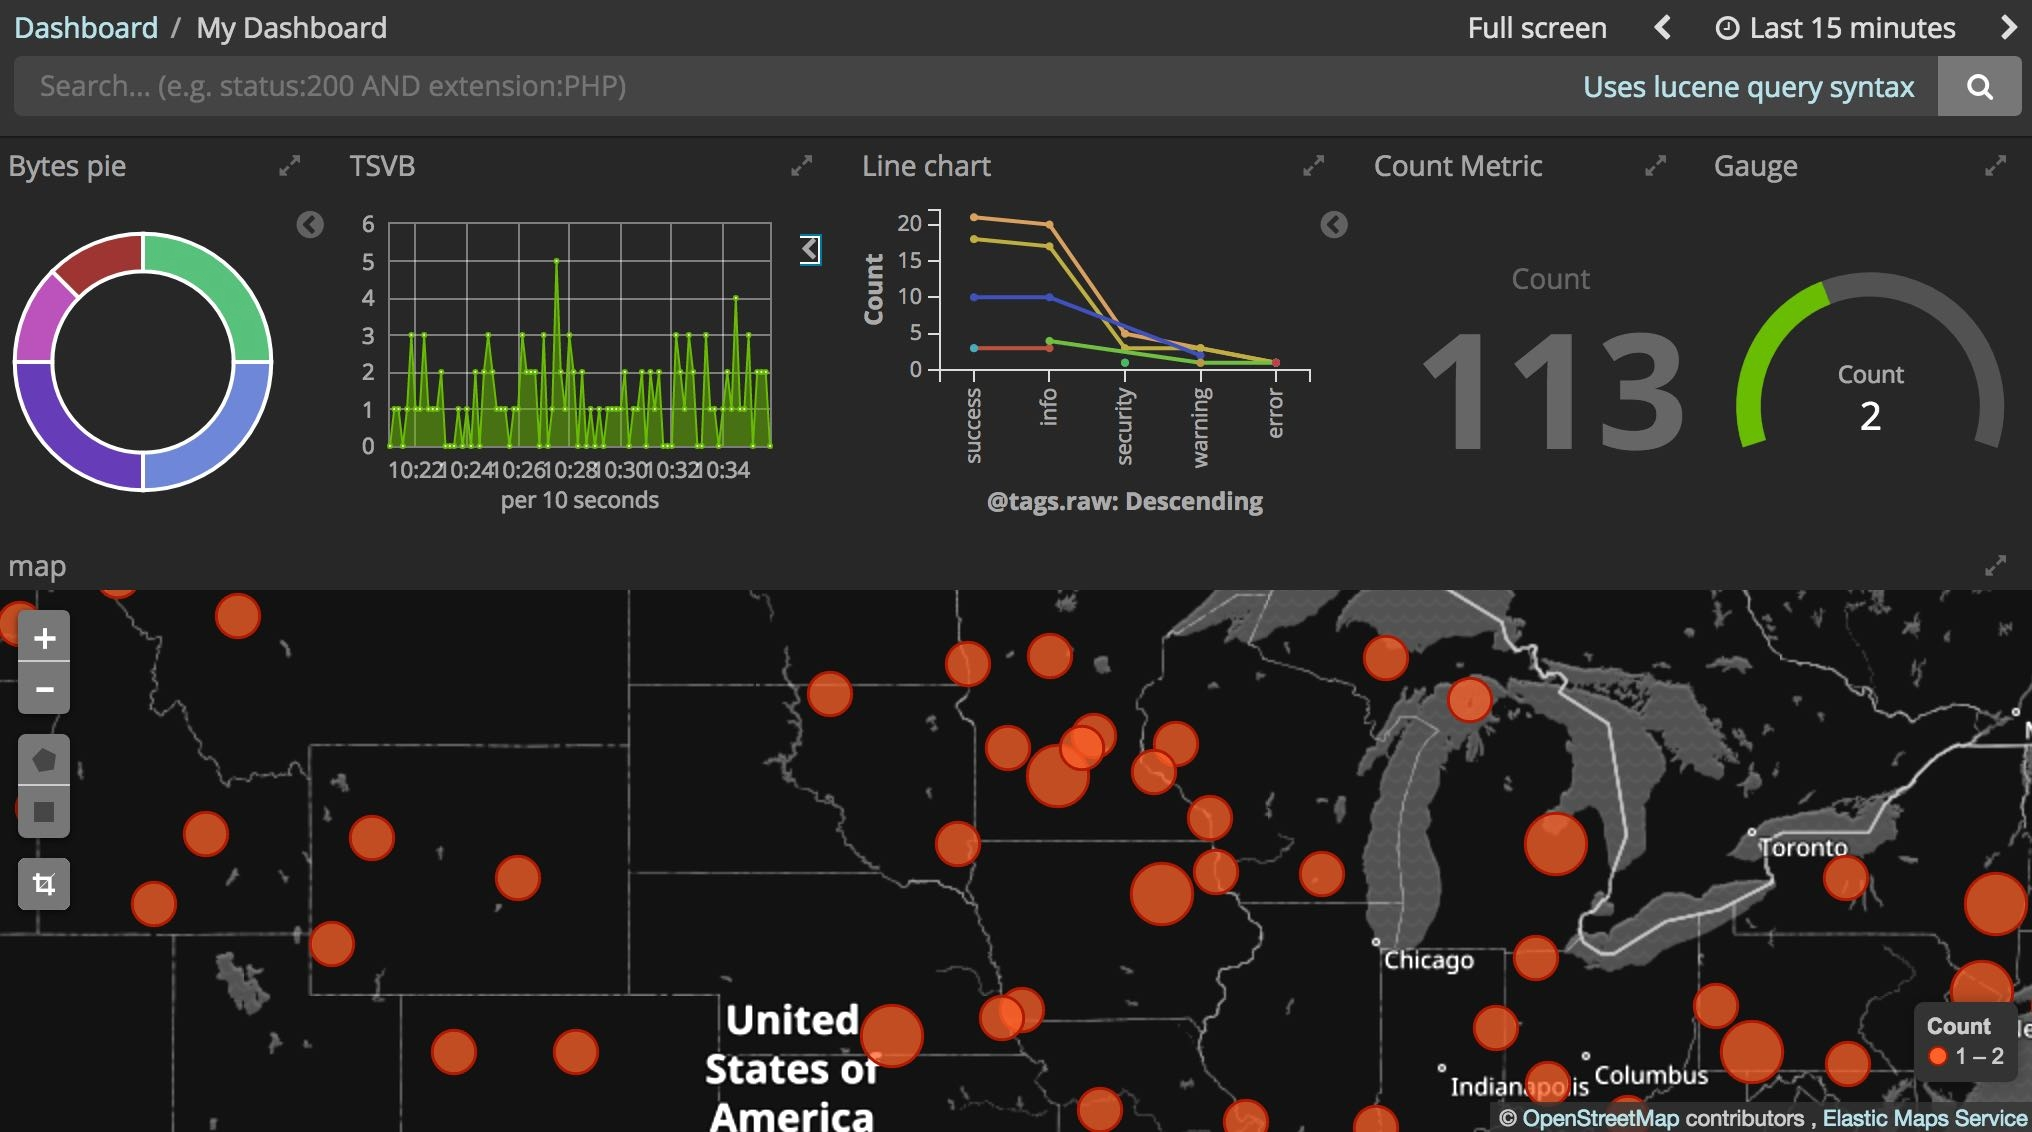
\includegraphics[width =\columnwidth]{dashboard_example5.png}
    \caption{Example 5}
    \label{fig:EX5}
\end{figure}
\begin{figure}[ht]
    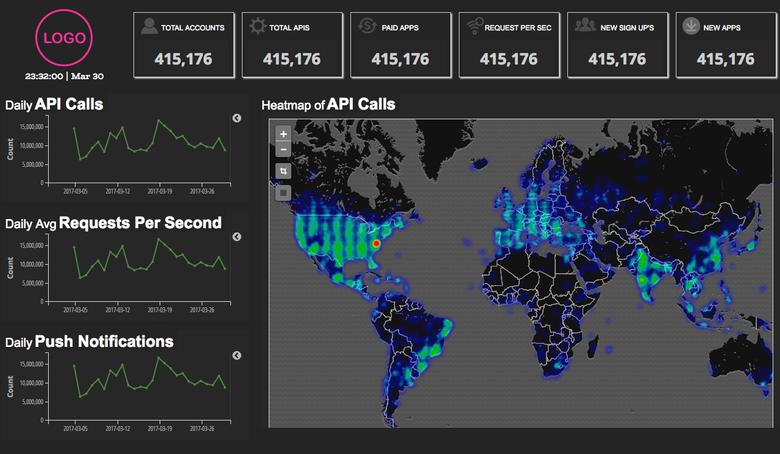
\includegraphics[width =\columnwidth]{dashboard_example6.png}
    \caption{Example 6}
    \label{fig:EX6}
\end{figure}

\chapter{Additional resources}
%%GITHUB REPO LINK 


\end{document}
